


% % Uncomment and use as if needed
% \newtheorem{theorem}{Theorem}
% \newtheorem{lemma}[theorem]{Lemma}
% \newtheorem{proposition}[theorem]{Proposition}
% \newtheorem{definition}[theorem]{Definition}
% \newdefinition{remark}{Remark}
% \newtheorem{corollary}[theorem]{Corollary}

% %----------------New Commands---------------%
% \newcommand{\innerprod}[1]{\left\langle #1 \right\rangle}
% \newcommand{\abs}[1]{\lvert #1 \rvert}
% \newcommand{\bigabs}[1]{\left \lvert #1 \right \rvert}

% \newcommand{\sobkp}[1]{W^{k,p}(#1)}
% \newcommand{\sob}{W^{k,p}}
% \newcommand{\Lloc}[1]{L_1^{loc}(#1)}
% \newcommand{\totalV}[1]{D_t^{\abs{#1}}V(t)}
% \newcommand{\totalJ}[1]{D_t^{\abs{#1}}J(t)}
% \newcommand{\D}{\textbf{D}}
% \newcommand{\fhat}{\hat{f}}

% %minGW
% \newcommand{\argminpsi}{\min\limits_{g(\textbf{w}(t),\psi(t))\in \sob}}

% %minSmoothGW
% \newcommand{\minSmoothGW}{\min\limits_{g(\textbf{w}(t),\delta(\psi(t)))\in \sob}}


% \let\WriteBookmarks\relax
% \def\floatpagepagefraction{1}
% \def\textpagefraction{.001}

% % Short title
% \shorttitle{}    

% % Short author
% \shortauthors{}  

% % Main title of the paper
% \title [mode = title]{The Effect of Architechture on Learning Behavior of Deep Neural Networks}  

% % Title footnote mark
% % eg: \tnotemark[1]
% %\tnotemark[1] 

% % Title footnote 1.
% % eg: \tnotetext[1]{Title footnote text}
% \tnotetext[1]{} 

% % First author
% %
% % Options: Use if required
% % eg: \author[1,3]{Author Name}[type=editor,
% %       style=chinese,
% %       auid=000,
% %       bioid=1,
% %       prefix=Sir,
% %       orcid=0000-0000-0000-0000,
% %       facebook=<facebook id>,
% %       twitter=<twitter id>,
% %       linkedin=<linkedin id>,
% %       gplus=<gplus id>]

% \author[1]{Allyson Hahn}%[<options>]]

% % Corresponding author indication
% \cormark[1]

% % Footnote of the first author
% \fnmark[1]

% % Email id of the first author
% \ead{}

% % URL of the first author
% \ead[url]{}

% % Credit authorship
% % eg: \credit{Conceptualization of this study, Methodology, Software}
% \credit{}

% % Address/affiliation
% \affiliation[1]{organization={Department of Mathematical Sciences, Northern Illinois University}}

% \author[2]{Krishnan Raghavan}%[]

% % Footnote of the second author
% \fnmark[2]

% % Email id of the second author
% \ead{}

% % URL of the second author
% \ead[url]{}

% % Credit authorship
% \credit{}

% % Address/affiliation
% \affiliation[2]{organization={Mathematics and Computer Science Division, Argonne National Laboratory}}

% % Footnote text
% \fntext[1]{}

% % For a title note without a number/mark
% %\nonumnote{}

% %-------------------Abstract-----------------------%
% \begin{abstract}
% We consider the effects of Neural Network architecture in the setting of continual learning. Using dynamic programming we complete a bilevel optimization to determine the optimal architecture for the current and previous task data followed by the optimal weights for the network. 
% \end{abstract}

% % Use if graphical abstract is present
% %\begin{graphicalabstract}
% %\includegraphics{}
% %\end{graphicalabstract}

% %-----------------Highlights------------------%
% \begin{highlights}
% \item The first quantification of NN architecture on the learning behavior
% \item Demonstrate the conditions to ensure stability of neural networks.
% \item A novel measure to efficiently perform neural architecture search and hyper-parameter search.
% \end{highlights}
% %-------------------Keywords-------------------%
% \begin{keywords}
%  Neural Network \sep Architecture Search\sep  \sep
% \end{keywords}
% \maketitle
 
\section{Introduction}
\textcolor{red}{Add motivation etc.}
\section{Literature Review}
\textcolor{red}{add Lit Review}
\section{Preliminaries}
These notation are adapted from \cite{kolda2009tensor}, please refer to the original paper for additional details. We begin by describing the notation for the paper. We use $\mathbb{N}$ to denote the set of natural numbers with $\mathbb{R}$ denoting the set of real numbers. We also use $\|.\|$ to denote the Euclidean norm for vectors, Frobenius norm for matrices.  Further, let $\innerprod{\cdot,\cdot}$ denote the dot product for vectors.  A $m^{th}$ order tensor is viewed as a multi-dimensional array contained in $\mathbb{R}^{I_1 \times I_2 \times I_3 \times I_4 \times \cdots I_{m}}$,  where the order can be thought of as the number of dimensions in the tensor. In this paper we will be mostly concerned with tensors of order $0, 1,2$ and $3$ which correspond to scalars, vectors and matrices and a list of matrices. Therefore, we will write a tensor of order $0$; a scalar, with lowercase letters, i.e., $x;$  a tensor of order one is denoted by lowercase bold alphabets such as $\bold{x}.$ A tensor of order $2$ is a matrix denoted by uppercase bold alphabets $\boldsymbol{X}$ and any tensor of order greater than $2$ are denoted by bolder Euler scripts letters such as $\boldsymbol{\mathcal{X}}.$ We will make one exception in our notation regarding the tensors that represent learnable/user defined parameters~(weights, architecture, step-size/learning rate, etc.), we will denote these with greek letters. The $i^{th}$ element of a vector $\bf{x}$ is denoted by $x_{[i]},$ while the $(i,j)^{th}$ element of a matrix $\boldsymbol{X}$ is denoted by $x_{[ij]}.$ Moreover, we denote the $i^{th}$ matrix in a tensor of order $3$ by $X_i.$  We will make the indices run from 1 to their capital letters such that $i = 1, \cdots, I.$ 

We consider the problem of continual learning for this paper. Continual learning is the problem of learning a sequence of tasks where each task is represented by a data set obtained at a task instance, i.e. $t \in \mathcal{T}, \mathcal{T} = \{0,1,\ldots, T\}.$ We will assume that the dataset~(a list of matrices/vectors/graphs) represented by $\boldsymbol{\mathcal{X}}(t)$ is provided at each task $t\in \mathcal{T},$ where $\boldsymbol{\mathcal{X}}(t)$ is sampled according to the distribution $\mathbb{P}$ where $\boldsymbol{\mathcal{X}}(t) \subset \mathcal{D}$ such that $\mathcal{D}$ -- the domain, is a measurable set with a non-empty interior. Moreover, $(\mathcal{D}, \mathcal{B}(\mathcal{D}), \mathbb{P})$ forms the probability triplet with $\mathcal{B}(\mathcal{D})$ being the Borel sigma algebra over the domain. 

The problem of interest to us is to understand the behavior of the neural network operator on a task such that the operator learns the new task in order to assimilate the new information on prior data. To this end, we will describe a neural network  as a member of the class of functions. We will let these classes of functions represent a Sobolev space.

\subsection{Neural Networks belong to a class of Sobolev space functions}
We let the class of functions the neural network may represent be contained in a Sobolev space with $k$ bounded derivatives. Our approach aligns with definitions provided in \cite{mahanNonclosednessSetsNeural2021a}.

\begin{definition}%\label{defn:sobo}
    Let $k \in \mathbb{N},$ $\mathcal{D}$ a measurable set with non-empty interior, and $1< p < \infty.$ Then, the Sobolev space $W^{k,p}(\mathcal{D})$ consists of all functions $h$ on $\mathcal{D}$ such that 
for all multi-indices $\alpha$ with $|\alpha| \leq k,$ the mixed partial derivative $\partial^{(\alpha)} h$ exists in the weak sense and belongs to $L^p(\mathcal{D})$. That is, 
    \[ W^{k,p}(\mathcal{D})  = \{ h \in L^p(\mathcal{D}) : \partial^{|\alpha|} h \in L^{p}(\mathcal{D}) \forall |\alpha| \leq k \}.\]
    The number $k$ is the order of the Sobolev space and the Sobolev space norm is defined as 
    \[ \| h\|_{W^{k,p}(\mathcal{D})} := \sum_{ |\alpha| \leq k } \| \partial^{|\alpha|} h \|_{L^{p}(\mathcal{D})}.\]
\end{definition}

To represent the class of functions described in Definition \ref{defn:sobo}, we will define a neural network as a function  $\fhat(w(t),  \psi(t) )$ with $d \in \mathbb{N}$ layers. In this notation of a neural network, $w(t)$ is comprised of all the weight parameters and $\psi(t)$ is comprised of the architecture and other user-defined parameters that are present in the neural network. Typically, the user-defined parameters are a combination of integer, categorical, and floating point values. We may therefore define
\begin{definition} %\label{defn:NN}
A $d$  layered neural network is given by an operator~(essentially a function) 
$\fhat(w(t), \psi(t) )\in W^{k,p}$ with $W^{k,p}$ being a Sobolev space. Furthermore, 
\begin{align}
  \fhat(w(t), \psi(t)) \big( . \big) & = \fhat_{d}(w_{d}(t), \psi_{d}(t)) \nonumber\\
                                 &\circ \fhat_{d-1}(w_{d-1}(t), \psi_{d-1}(t)) \nonumber\\
                                &\vdots\nonumber \\
                                &\circ \fhat_{2}(w_{2}(t), \psi_{2}(t))\nonumber \\
                                &\circ \fhat_{1}(w_{1}(t), \psi_{1}(t)) \big( . \big)                 
\end{align}
describes the layerwise compositions and $\big( . \big)$ represents the input tensor to which the operator is applied.
\end{definition}
Note that this definition of neural networks can be used to define feedforward neural networks, recurrent, convolutional and even graph neural networks or a combination of the three. 
The distinction will come from how each layerwise composition is defined with this setup. Therefore, any analysis from this point will describe the behavior of 
all types of networks. Moreover, the parameters corresponding to the architecture are assumed to be a function of $t.$ As we cannot determine derivatives of discrete with respect to parameters in the classical sense (i.e. derivative of $\psi(t)$) this setup is provided to perform optimization
on both the architecture and the weights of the neural network model by utilizing the notion of derivatives in the weak sense.

To describe the neural network training mechanism and the learning problem. We first describe the ideal function that must be approximated.

 \begin{definition}%\label{defn:NN_learning}
        Let $f(t)\in W^{k,p}(\mathcal{D})$ for all $t\in \{0,\ldots, T\}$ denote the \textit{target function} which is to be approximated. If $\hat{f}(w(t),\psi(t))$ denotes a neural network determined to approximate $f(t)$ at task $t,$ then the \textit{loss function} (or error of approximation) for $x\in \mathcal{X}(t)$ is given by 
        \begin{align*}
            \ell(\fhat(w(t),\psi(t)))(x) &=\\
            &\| \fhat(w(t),\psi(t))(x)-f(t)(x)\|_{W^{k,p}(\mathcal{D})}.
        \end{align*} 
    \end{definition}
The function $f$ in the context of ML is an ideal forecasting model that can forecast temperature perfectly or an ideal classification model that performs some classification problem.

\begin{remark}
    In application, we will assume $\mathcal{D}$ is compact to guarentee the target function $f(t)$ exists in a Sobolev space $W^{k,p}(\mathcal{D}),$ by Corollary 3.5. in \cite{mahanNonclosednessSetsNeural2021a}. However, in the event compactness cannot be assumed, we find the minimum norm solution to the problem in the Sobolev space.
\end{remark}


\subsection{Understanding the impact of similar and dissimilar tasks}
For illustration, consider Fig.~\ref{fig:CL1}, there are three tasks shown to the model in order with a fixed architecture, denoted by $\psi(1).$
\begin{figure}
    \centering
    \includegraphics[width=1.1\linewidth]{Figures/CL1.png}
    \caption{The basic problem of Continual Learning}
    %\label{fig:CL1}
\end{figure}
The goal is to find the optimal weights for the NN at each task which allow it to perform accurately on both the current task and all previous tasks. However, determining the optimal weights is highly dependent on each task's data. Intuitively, if the data in task $\boldsymbol{\mathcal{X}}(t)$ is similar to $\boldsymbol{\mathcal{X}}(t+1),$ we can find a NN $\hat{f}$ which  learns the new task and transfers learning from the previous tasks. But, if the data in the tasks are too dissimilar, we may or may not be able to find a NN solution. To make this more precise, consider Fig. \ref{fig:challenge}.
\begin{figure}
    \centering
    \includegraphics[width=\linewidth]{Figures/problem1.png}
    \caption{The actual problem}
    %\label{fig:challenge}
\end{figure}
 Let $\mathcal{F}_t = \{\fhat(w,\psi)\in W^{k,p}\}$ represent the search space for the set of all possible NN solutions for learning task $t.$ Note that this is indeed contained in a Sobolev space. In Fig. \ref{fig:challenge}, we can view each search space as a ball. Then, each \ding{58} represents the NN solution for only the ball $\mathcal{F}_t.$ We want a transfer of learning across all tasks, so the NN solution we desire must lie in the intersection of the search space for the new task and the search space for all previous tasks. This is represented in Fig. \ref{fig:challenge} by the $\smiley{}$ at each step. During this process, we can quickly be met with a problem, as the intersection of the search spaces is not required to be nonempty. However, before proposing a solution to issue, we solidify the idea that we can find a solution when tasks data is similar. Toward that end, consider the following definition.
 
 %definition of continuous w.r.t measure
     \begin{definition}
 %\label{defintersect}
     Let $\overline{\mathcal{X}} = \bigcup_{t=0}^\infty \mathcal{X}(t)$ with the power set $\mathcal{P(\overline{X})}$ as its topology. Set $\mathcal{B(\overline{X})}$ to be the Borel sigma algebra on $\overline{\mathcal{X}}$ equipped with a probability measure denoted $\mu.$ Then, $(\overline{\boldsymbol{\mathcal{X}}},\mathcal{B}(\overline{\boldsymbol{\mathcal{X}}}), \mu)$ forms a probability measure space. Let $g:\overline{\boldsymbol{\mathcal{X}}}\rightarrow \mathbb{R}$ be a measurable function, and set $F:\mathcal{B}(\overline{\boldsymbol{\mathcal{X}}})\rightarrow \mathbb{R}$ to be the function
     \begin{align*}
         F(A) & = \int_A g(x)d\mu.
     \end{align*}
     Then, we say $F$ is \textit{continuous with respect to the measure} if for every $\varepsilon>0,$ there exists $\delta >0$ such that $\abs{F(A)-F(B)} < \varepsilon$
     whenever $A,B\in \mathcal{B(\overline{X})}$ such that $\mu(A\bigtriangleup B)<\delta.$
 \end{definition}
Definition \ref{defintersect} can be deduced from basic measure theory results found in \cite{weaver2013measure}. The intuition behind this definition is that sets which are similar (with respect to measure) will result in integrals of $\hat{f}$ over the respective sets which are close in value. In the set theory context, the notation $A\bigtriangleup B$ represents set symmetric difference, which describes the elements two sets do not share, see Fig. \ref{fig:setsim}. Thus, as $\mu(A\bigtriangleup B)$ gets larger, the size of the intersection space (i.e. $\mu(A\cap B)$) shrinks. Hence, the measure of the set symmetric difference provides a notion of how ``similar" how ``different" two sets are.
\begin{figure}
    \centering
    \scalebox{.8}{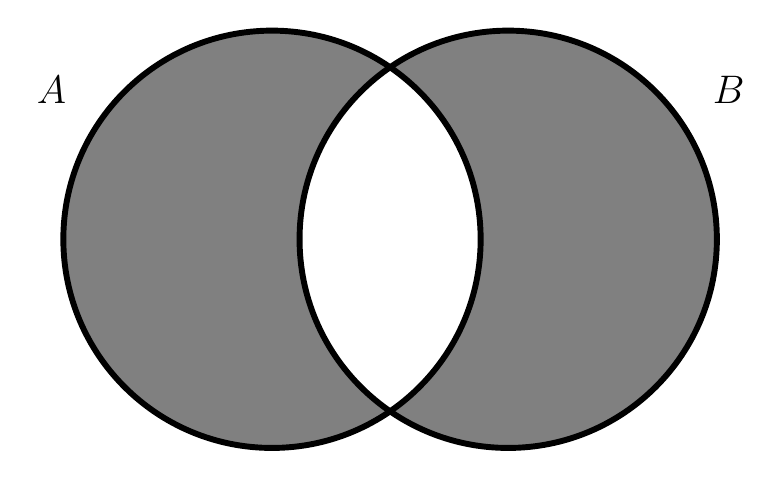
\begin{tikzpicture}
        \def\firstcircle{(-.5,0) circle (2.65cm)}
        \def\secondcircle{(2.5,0) circle (2.65cm)}
        
        % Fill the symmetric difference
        \fill[even odd rule, gray]\firstcircle \secondcircle;
        
        % Draw the circle outlines and add labels
        \draw[draw=black,line width=.75mm] \firstcircle;
        \draw[draw = black, line width=.75mm] \secondcircle;
        \node at (-3.3,1.9) {\Large$A$};
        \node at (5.3,1.9) {\Large$B$};
    \end{tikzpicture}}
    \caption{The gray shaded region represents set symmetric difference $A\bigtriangleup B.$}
    %\label{fig:setsim}
\end{figure}

Then, the theorem below describes that tasks with similar data will result in similar values for the integral of the loss function. If the expected value function is continuous with respect to measure, then we can choose $\varepsilon >0$ small and find a $\delta >0$ such that $\abs{E(\mathcal{X}(t))-E(B)}<\varepsilon$ for all $B$ such that $\mu(\mathcal{X}(t)\bigtriangleup B)<\delta.$ Thus, if two tasks $\mathcal{X}(t)$ and $\mathcal{X}(t+\Delta t)$ are similar (i.e. $\mu(\mathcal{X}(t)\bigtriangleup \mathcal{X}(t+\Delta t))<\delta)$, then the loss values are similar (i.e. $\abs{E(\mathcal{X}(t))-E(\mathcal{X}(t+\Delta t))}<\varepsilon$).

%theorem proving EV is cont. w.r.t. meausre
\begin{theorem}%\label{contMeasure}
    Let $(\overline{\boldsymbol{\mathcal{X}}},\mathcal{B}(\overline{\boldsymbol{\mathcal{X}}}), \mu)$ be the measure space as defined above. Then, the expected value function:
    \begin{align}
        E(A) = \int_A \ell((\fhat(w,\psi))(x))d\mu
    \end{align}
    is continuous with respect to the measure.
\end{theorem}

\begin{proof}
    We can assume that the loss function $\ell$ is continuous and bounded across all tasks. Suppose that the constant $M_0>0$ is the value which bounds $\ell$ on every task. Let $\varepsilon>0$ and  set $\delta = \varepsilon/M_0.$ Further let $A,B\in \mathcal{\mathcal{B}}(\mathcal{X})$ such that $\mu(A\bigtriangleup B)< \delta.$ By disjoint additivity of $\mu$ and triangle inequality, 
    \begin{align*}
        \abs{E(A) -E(B)} & = \Big\vert\int_A \ell(\fhat(w,\psi)(x))d\mu\\
        & \hspace{10mm}- \int_B\ell(\fhat(w,\psi)(x))d\mu\Big\vert\\
        & = \Big\vert\int_{A\setminus B} \ell(\fhat(w,\psi)(x))d\mu\\
        &\hspace{10mm} + \int_{A\cap B} \ell(\fhat(w,\psi)(x))d\mu\\
        & \hspace{10mm}-\int_{B\setminus A}\ell(\fhat(w,\psi)(x))d\mu\\
        & \hspace{10mm}-\int_{A\cap B}\ell(\fhat(w,\psi)(x))d\mu\big\vert\\
        & \leq \int_{A\setminus B} \abs{\ell(\fhat(w,\psi)(x))}d\mu\\
        & \hspace{10mm}+\int_{B\setminus A}\abs{\ell(\fhat(w,\psi)(x))}d\mu.
    \end{align*}
    Then, by the boundedness of $\ell,$
    \begin{align*}
        \int_{A\setminus B} \abs{\ell(\fhat(w,\psi)(x))}d\mu+\int_{B\setminus A}\abs{\ell(\fhat(w,\psi)(x))}d\mu\\
        \leq M_0\mu(A\setminus B) + M_0\mu(B\setminus A).
    \end{align*}
    Hence,
    \begin{align*}
        M_0\mu(A\setminus B) + M_0\mu(B\setminus A) & = M_0(\mu(A\setminus B) + \mu(B\setminus A))\\
        & = M_0\mu(A\bigtriangleup B)\\
        & < M_0 \delta\\
         & = M_0 \frac{\varepsilon}{M_0}\\
         & = \varepsilon,
    \end{align*}
    as desired.
\end{proof}

%remark justifying loss bounded on all tasks
\begin{remark}%\label{boundedremark}
    It is clear that $\ell$ is bounded on each individual task with bound $M_i$ for tasks $i\in \mathbb{N}.$ However, it is reasonable to also assume that there is some constant $M_0<\infty$ for which $M_i\leq M_0$ for all $i\in \mathbb{N}$ because if one did not exist then the problem would be unsolvable. 
\end{remark}

Theorem \ref{contMeasure} solidifies the notion that similar tasks produce similar loss values. In return, this implies the intersection search space for finding a NN is non-empty. Moreover, the contrapositive reveals that dissimilar loss values imply dissimilar tasks. However, it cannot be shown for an arbitrary continual learning problem that dissimilar tasks result in dissimilar loss values. In other words, we do not know if the intersection search space will always be nonempty. In terms of our previous result, this says if $\varepsilon>0$ is small then we know there exists $\delta >0$ such that $\abs{E(A)-E(B)}<\varepsilon$ for all $A,B$ satisfying $\mu(A\bigtriangleup B)< \delta.$ But, if we have two tasks $\mathcal{X}(t)$ and $\mathcal{X}(t+\Delta t)$ such that $\mu(\mathcal{X}(t)\bigtriangleup \mathcal{X}(t+\Delta t))\geq \delta$ the we do not know whether $\abs{E(\mathcal{X}(t))-E(\mathcal{X}(t+\Delta t)}<\varepsilon$ (i.e. similar loss values) or $\abs{E(\mathcal{X}(t))-E(\mathcal{X}(t+\Delta t)}\geq\varepsilon$ (i.e. dissimilar loss values).

Now that we see the relationship between similarity of tasks and size of the intersection of the corresponding solution spaces, let us determine what to do when dissimilar tasks produce dissimilar loss values, and hence a shrinking intersection space. The goal is to increase the similarity in expected values for two tasks. Toward this end, we consider what impacts the expected value.

First, suppose we fix the architecture for each task. Then, we can find the following lower bound on the gradient of the expected value function. For sake of notation, set
\begin{align*}
    \|\nabla E\| & = \lim_{\Delta t\rightarrow 0} \frac{\abs{E(\boldsymbol{\mathcal{X}}(t)))-E(\boldsymbol{\mathcal{X}}(t+\Delta t))}}{\Delta t}.
\end{align*}
to represent the norm of the gradient of the expected value.

    \begin{theorem}%\label{lowerboundTheoremw}
    Suppose $\boldsymbol{\mathcal{X}}(t)$ and $\boldsymbol{\mathcal{X}}(t+1)$ are two consecutive tasks in the measure space $(\overline{\boldsymbol{\mathcal{X}}}, \mathcal{B}(\overline{\boldsymbol{\mathcal{X}}}),\mu).$ Let $L_1>0$ and $0\leq \delta\leq 1$ all be constants. Set $M_0$ to be the upperbound on the loss function $\ell$ across all tasks. Moreover, suppose $\psi(t) = \psi(1)$ for all tasks $t.$ Then, for $\mu(\boldsymbol{\mathcal{X}}(t)\bigtriangleup \boldsymbol{\mathcal{X}}(t+1))\geq \delta,$ the following holds
    \begin{align}
        \|\nabla E\| &\geq M_0\delta - L_1\abs{\Delta w}\displaystyle\int_{\boldsymbol{\mathcal{X}}(t)} \|\partial^1_w \hat{f}(w(t),\psi(1))\|_{L^p}d\mu. % %\label{lowerw}
    \end{align}
\end{theorem}

The lower bound in (\ref{lowerw}) confirms that the norm of the gradient is dependent upon the bound on the loss function and the change in the weights. In particular, we see that the more we change the weights $w(t),$ the smaller our lower bound gets. As a smaller norm of the gradient implies a smaller change in the expected value between two tasks (i.e. smaller $\abs{E(\boldsymbol{\mathcal{X}}(t)))-E(\boldsymbol{\mathcal{X}}(t+\Delta t))}$), it is clear that we could reduce the lower bound in (\ref{lowerw}) by changing the weights. However, we can only change the weights so far before overfitting occurs. In other words, there is a bound on the change in weights, and hence a bound on much we can reduce the lower bound (\ref{lowerw}). It would be ideal if the lower bound could be reduced further. 

It is important to note that in Theorem \ref{lowerboundTheoremw}, we fix the architecture.  What if we allow for changing the architecture as well? Intuitively, we know changing the architecture via some architecture search will result in a better performing NN (i.e. smaller expected value). However, let us provide a concrete proof to support this intuition. The following theorem provides us with a lower bound on $\|\nabla E\|$ that is smaller than that presented in (\ref{lowerw}). Thus, we have the potential to reduce $\|\nabla E\|$ and hence reduce the change in the expected value $\abs{E(\boldsymbol{\mathcal{X}}(t)))-E(\boldsymbol{\mathcal{X}}(t+\Delta t))}.$ 

%theorem 
\begin{theorem}%\label{lowerBoundpsi}
    Suppose $\boldsymbol{\mathcal{X}}(t)$ and $\boldsymbol{\mathcal{X}}(t+1)$ are two consecutive tasks in the measure space $(\overline{\boldsymbol{\mathcal{X}}}, \mathcal{B}(\overline{\boldsymbol{\mathcal{X}}}),\mu).$ Let $L_1>0$ and $0\leq \delta\leq 1$ all be constants. Set $M_0$ to be the upperbound on the loss function $\ell$ across all tasks. Then, for $\mu(\boldsymbol{\mathcal{X}}(t)\bigtriangleup \boldsymbol{\mathcal{X}}(t+1))\geq \delta,$ the following holds
    \begin{align}
        \abs{\nabla E} &\geq M_0\delta\nonumber\\
        & - L_1\abs{\Delta w}\displaystyle\int_{\boldsymbol{\mathcal{X}}(t)} \|\partial^1_w \hat{f}(w(t,\psi),\psi(t))\|_{L^p}d\mu\nonumber\\
        & - L_1\abs{\Delta \psi}\displaystyle\int_{\boldsymbol{\mathcal{X}}(t)} \|\partial^1_\psi \hat{f}(w(t,\psi),\psi(t))\|_{L^p}d\mu.%\label{lowerpsi}
    \end{align}
\end{theorem}

\begin{proof}
Recall that
    \begin{align}
        \abs{\nabla E(\boldsymbol{\mathcal{X}}(t))} & = \lim_{\Delta t\rightarrow 0} \frac{\abs{E(\boldsymbol{\mathcal{X}}(t))-E(\boldsymbol{\mathcal{X}}(t+\Delta t))}}{\Delta t}.%\label{grad}
    \end{align}
    We begin with the numerator of (\ref{grad}). The first-order Taylor series expansion of $E(\boldsymbol{\mathcal{X}}(t+\Delta t))$ about  $t,$ is given by
    \begin{align}
        E(\boldsymbol{\mathcal{X}}(t+\Delta t)) & = E(\boldsymbol{\mathcal{X}}(t)) + \Delta t\Big[ E_{\boldsymbol{\mathcal{X}}} (\boldsymbol{\mathcal{X}}(t)\Delta \boldsymbol{\mathcal{X}}(t+\Delta t))\\
        & + E_w(\boldsymbol{\mathcal{X}}(t)) + E_\psi(\boldsymbol{\mathcal{X}}(t))\Big] + o(\Delta t),%\label{taylorexp}
    \end{align}
    where $E_{\boldsymbol{\mathcal{X}}} , E_w,$ and $E_\psi$ are the partial derivatives of the expected value function with respect to the data, weights, and architecture, respectively. Now, we work on acquiring each partial derivative. Toward that end, 
    \begin{align}
        E_{\boldsymbol{\mathcal{X}}} (\boldsymbol{\mathcal{X}}(t)\Delta \boldsymbol{\mathcal{X}}(t+\Delta t)) & =\mu( \boldsymbol{\mathcal{X}}(t)\Delta \boldsymbol{\mathcal{X}}(t+\Delta t))\\
        & \cdot \displaystyle\int_{\boldsymbol{\mathcal{X}}(t)\Delta \boldsymbol{\mathcal{X}}(t+\Delta t)} \ell(\hat{f}(w,\psi))d\mu.%\label{E_X1}
    \end{align}
    To determine the remaining two derivatives, we use the Sobolev function chain rule found in \cite{evans2022partial}. We can do so as $\ell$ is real-valued and bounded, and $\ell'$ is continuously differentiable. Then,
    \begin{align}
        E_w (\boldsymbol{\mathcal{X}}(t)) & = \displaystyle\int_{\boldsymbol{\mathcal{X}}(t)} \ell'(\hat{f}(w,\psi))\cdot \partial_w^1 \hat{f}(w,\psi)\cdot \Delta w \hspace{1mm}  d\mu.%\label{E_w},\\
        E_\psi (\boldsymbol{\mathcal{X}}(t)) & = \displaystyle\int_{\boldsymbol{\mathcal{X}}(t)} \ell'(\hat{f}(w,\psi))\cdot \partial_\psi^1 \hat{f}(w,\psi)\cdot \Delta \psi \hspace{1mm}  d\mu.%\label{E_psi}
    \end{align}
    Substituting (\ref{E_X1}), (\ref{E_w}), and (\ref{E_psi}) into the Taylor series expansion (\ref{taylorexp}), we have
    \begin{align*}
        E(\boldsymbol{\mathcal{X}}(t+\Delta t)) & = E(\boldsymbol{\mathcal{X}}(t)) + \Delta t\Big[\mu( \boldsymbol{\mathcal{X}}(t)\Delta \boldsymbol{\mathcal{X}}(t+\Delta t))\\
        & \cdot \displaystyle\int_{\boldsymbol{\mathcal{X}}(t)\Delta \boldsymbol{\mathcal{X}}(t+\Delta t)} \ell(\hat{f}(w,\psi))d\mu\\
        & + \displaystyle\int_{\boldsymbol{\mathcal{X}}(t)} \ell'(\hat{f}(w,\psi))\cdot \partial_w^1 \hat{f}(w,\psi)\cdot \Delta w \hspace{1mm}  d\mu\\
        & +\displaystyle\int_{\boldsymbol{\mathcal{X}}(t)} \ell'(\hat{f}(w,\psi))\cdot \partial_\psi^1 \hat{f}(w,\psi)\cdot \Delta \psi \hspace{1mm}  d\mu\Big]\\
        & + o(\Delta t).
    \end{align*}
    Now substituting the Taylor series expansion into our original expression we have
    \begin{align*}
        |\nabla E(\boldsymbol{\mathcal{X}}(t))| & =  \lim_{\Delta t\rightarrow 0} \frac{\abs{E(\boldsymbol{\mathcal{X}}(t+\Delta t))-E(\boldsymbol{\mathcal{X}}(t))}}{\Delta t}\\
        & = \lim_{\Delta t\rightarrow 0} \Big\vert \mu( \boldsymbol{\mathcal{X}}(t)\Delta \boldsymbol{\mathcal{X}}(t+\Delta t))\\
        & \cdot \displaystyle\int_{\boldsymbol{\mathcal{X}}(t)\Delta \boldsymbol{\mathcal{X}}(t+\Delta t)} \ell(\hat{f}(w,\psi))d\mu\\
        & + \displaystyle\int_{\boldsymbol{\mathcal{X}}(t)} \ell'(\hat{f}(w,\psi))\cdot \partial_w^1 \hat{f}(w,\psi)\cdot \Delta w \hspace{1mm}  d\mu\\
        & + \displaystyle\int_{\boldsymbol{\mathcal{X}}(t)} \ell'(\hat{f}(w,\psi))\cdot \partial_\psi^1 \hat{f}(w,\psi)\cdot \Delta \psi \hspace{1mm} d\mu\Big\vert.
    \end{align*}
    By reverse triangle inequality in \cite{pons2014real},
    \begin{align*}
        |\nabla E(\boldsymbol{\mathcal{X}}(t))| & \geq \lim_{\Delta t\rightarrow 0} \mu( \boldsymbol{\mathcal{X}}(t)\Delta \boldsymbol{\mathcal{X}}(t+\Delta t))\\
        & \cdot \bigabs{\displaystyle\int_{\boldsymbol{\mathcal{X}}(t)\Delta \boldsymbol{\mathcal{X}}(t+\Delta t)} \ell(\hat{f}(w,\psi))d\mu}\\
        & - \bigabs{\displaystyle\int_{\boldsymbol{\mathcal{X}}(t)} \ell'(\hat{f}(w,\psi))\cdot \partial_w^1 \hat{f}(w,\psi)\cdot \Delta w \hspace{1mm}  d\mu}\\
        & - \bigabs{\displaystyle\int_{\boldsymbol{\mathcal{X}}(t)} \ell'(\hat{f}(w,\psi))\cdot \partial_\psi^1 \hat{f}(w,\psi)\cdot \Delta \psi \hspace{1mm} d\mu}.
    \end{align*}
    By integral properties in \cite{weaver2013measure}, notice
    \begin{align*}
        |\nabla E(\boldsymbol{\mathcal{X}}(t))| & \geq \lim_{\Delta t\rightarrow 0} \mu( \boldsymbol{\mathcal{X}}(t)\Delta \boldsymbol{\mathcal{X}}(t+\Delta t))\\
        &\cdot \bigabs{\displaystyle\int_{\boldsymbol{\mathcal{X}}(t)\Delta \boldsymbol{\mathcal{X}}(t+\Delta t)} \ell(\hat{f}(w,\psi))d\mu}\\
        & - \displaystyle\int_{\boldsymbol{\mathcal{X}}(t)} \abs{\ell'(\hat{f}(w,\psi))}\cdot \|\partial_w^1 \hat{f}(w,\psi)\|_{L^p}\cdot \abs{\Delta w} \hspace{1mm}  d\mu\\
        & - \displaystyle\int_{\boldsymbol{\mathcal{X}}(t)} \abs{\ell'(\hat{f}(w,\psi))}\cdot \|\partial_\psi^1 \hat{f}(w,\psi)\|_{L^p}\cdot \abs{\Delta \psi} \hspace{1mm} d\mu.
    \end{align*}
     We can assume that the loss function $\ell$ and its derivative $\ell'$ are bounded above by constants $M_0$ and $L_1$ respectively. Thus, by integral properties in \cite{weaver2013measure}
    \begin{align*}
        |\nabla E(\boldsymbol{\mathcal{X}}(t))| & \geq \lim_{\Delta t\rightarrow 0} \mu( \boldsymbol{\mathcal{X}}(t)\Delta \boldsymbol{\mathcal{X}}(t+\Delta t))\cdot M_0\\
        & - L_1 \displaystyle\int_{\boldsymbol{\mathcal{X}}(t)}\|\partial_w^1 \hat{f}(w,\psi)\|_{L^p}\cdot \abs{\Delta w} \hspace{1mm}  d\mu\\
        & - L_1\displaystyle\int_{\boldsymbol{\mathcal{X}}(t)}\|\partial_\psi^1 \hat{f}(w,\psi)\|_{L^p}\cdot \abs{\Delta \psi} \hspace{1mm} d\mu.
    \end{align*}
    Finally, as we assumed $\mu( \boldsymbol{\mathcal{X}}(t)\Delta \boldsymbol{\mathcal{X}}(t+\Delta t))\geq \delta$ and $\Delta w$ and $\Delta \psi$ are independent of the data, we have
    \begin{align*}
        |\nabla E(\boldsymbol{\mathcal{X}}(t))| & \geq M_0\delta\\
        & - L_1 \abs{\Delta w} \displaystyle\int_{\boldsymbol{\mathcal{X}}(t)}\|\partial_w^1 \hat{f}(w,\psi)\|_{L^p}\hspace{1mm}  d\mu\\
        & - L_1\abs{\Delta \psi}\displaystyle\int_{\boldsymbol{\mathcal{X}}(t)}\|\partial_\psi^1 \hat{f}(w,\psi)\|_{L^p} d\mu,
    \end{align*}
    as desired.
\end{proof}

The previous theorem provided us with a lower bound (\ref{lowerpsi}) which was inherently small than (\ref{lowerw}) since we now can subtract the change in the architecture $\psi(t)$ as well as the change in the weights $w(t).$  This leads us to the following corollary.

\begin{corollary}%\label{archCor}
    Suppose $\boldsymbol{\mathcal{X}}(t)$ and $\boldsymbol{\mathcal{X}}(t+\Delta t)$ are two consecutive tasks in the measure space $(\overline{\boldsymbol{\mathcal{X}}}, \mathcal{B}(\overline{\boldsymbol{\mathcal{X}}}), \mu).$ Let $\mu(\boldsymbol{\mathcal{X}}(t)\bigtriangleup \boldsymbol{\mathcal{X}}(t+\Delta t))\geq \delta$ for $0<\delta \leq 1.$ The architecture $\psi$ of a network can be changed to absorb the impact of $\mu(\boldsymbol{\mathcal{X}}(t)\bigtriangleup \boldsymbol{\mathcal{X}}(t+\Delta t))\geq \delta.$
\end{corollary}


\begin{proof}
Let $\varepsilon >0$ small. Since the expected value function is continuous with respect to measure by Theorem \ref{contMeasure}, we can find a corresponding $\delta>0.$ Suppose we have two tasks $\boldsymbol{\mathcal{X}}(t)$ and $\boldsymbol{\mathcal{X}}(t+\Delta t))$ for which $\mu(\boldsymbol{\mathcal{X}}(t)\bigtriangleup \boldsymbol{\mathcal{X}}(t+\Delta t))\geq \delta.$ Moreover, suppose $\abs{E(\boldsymbol{\mathcal{X}}(t+\Delta t))-E(\boldsymbol{\mathcal{X}}(t))}\geq \varepsilon.$ Then, by Theorem \ref{lowerBoundpsi}, we see that changing the architecture and training on a new optimal architecture that we can have
    \begin{align*}  
    \abs{\nabla E(\boldsymbol{\mathcal{X}}(t))}& \geq M_0\delta\\
    & - L_1\abs{\Delta w}\displaystyle\int_{\boldsymbol{\mathcal{X}}(t)} \|\partial^1_w \hat{f}(w(t,\psi),\psi(t))\|_{L^p}d\mu\\
    & - L_1\abs{\Delta \psi}\displaystyle\int_{\boldsymbol{\mathcal{X}}(t)} \|\partial^1_\psi \hat{f}(w(t,\psi),\psi(t))\|_{L^p}d\mu.%\label{eq:final}
    \end{align*}
Thus, changing the architecture of the network can offset the impact of consecutive tasks whose data differ substantially.
\end{proof}

With the knowledge of Corollary \ref{archCor}, we offer a solution to the issue of a vanishing intersection. In particular, we propose a method that allows us to change the size of the intersection space by introducing capacity, via hyper parameters, guarenteeing the intersection search space will be nonempty. We provide a brief overview of the method here for the reader to gain familiarity before diving into the mathematics of this process in the next section.\\

As depicted in Fig. \ref{fig:solution},
rather than fixing the architecture at $\psi^*$ for all tasks, allowing an architecture search at each step affords us the opportunity for a larger intersection space, as proven in Corollary \ref{archCor}. 
\begin{figure}
    \centering
    \includegraphics[width=\linewidth]{Figures/intersect22.png}
    \caption{The Solution, where we change the size of the intersection space by introducing more capacity, through choosing novel hyperparameters}
    %\label{fig:solution}
\end{figure}
To understand how this is accomplished, consider Fig. \ref{fig:method}, which describes the method for the first and second task. We begin at task $t = 1$ and determine an optimal weight denoted $w^*(1) = w^\infty(1).$ This gives us a NN solution in $\mathcal{F}_1.$ Then, we perform a derivative free hyper-parameter search on the architecture. The solution to this search is denoted $\psi^\infty(2).$ Using this new optimal architecture we complete what we call ``Low Rank Transfer" on the previous task's optimal weights, accomplishing a transfer of learning. This produces $g(w^N(2),\psi^\infty(2)).$ Then, we train on the next data task producing a NN solution $g(w^\infty(2),\psi^\infty(2))$ which is optimal for both the first and second task. In the process of Low Rank Transfer, we guarantee transfer of learning, allowing for the intersection of the NN search spaces for the task one and task two increase. Continuing to complete this process for all tasks will require the intersection $\cap_{i=1}^t \mathcal{F}_i$ to be nonempty.
\begin{figure}
    \centering
    \includegraphics[width=1.1\linewidth]{Figures/method.png}
    \caption{How we do this?}
    %\label{fig:method}
\end{figure}

\subsection{NN-Based Learning Problem}
In the CL setting, we design a regime which will be able to learn a target function. Thus, we seek to approximate the target function $f(t),$ with a small error. This error can be described by the loss function $\ell,$ as described in Definition \ref{defn:NN_learning}. It is then calculated as an expected value in the data, as defined in Theorem \ref{contMeasure}. More specifically Specifically, we write the expected value in terms of data, weights, and architecture, as below
\begin{align*}
    J(w(t),\psi(t),\boldsymbol{\mathcal{X}}(t)) & = \int_0^\tau \ell(g(w(t),\psi(t))(X(q)))dq
\end{align*}
A traditional learning structure seeks to minimize the cost $J(t)$ through an iterative 
procedure that drives $J(t) \rightarrow 0$ as $t \rightarrow \infty.$ Moreover, this learning 
structure is also mathematically guaranteed to converge with standard optimizers such as 
Adam~\cite{kingmaAdamMethodStochastic2017}. A typical learning process for these approaches 
involve extracting batches of data from $\boldsymbol{\mathcal{X}}(t)$ and then updating the network 
based on these batches of data. All of these updates are performed with a fixed architecture. 

The traditional learning process provides two key insights. First, the learning process is always done with a fixed architecture. 
Second, there is a cumulative impact of batches of data on the learning problem. The convergence of a neural network should be shown 
by demonstrating that the cumulative effect of these batches of data exhibits a pointwise convergence. Although, in standard proofs
of gradient-based approaches, the cumulative effect is considered by defining a series of gradients and then summing across gradients,
the analysis structure is still performed assuming a fixed architecture. 

As seen in the previous section, we are instead considering a scenario when the architecture and the model parameters are learned. Subsequently, we will precisely quantify the effects of the model, the data, and the architecture on the learning problem.

Towards this end, we begin by writing a cumulative learning problem for learning both the weights and the architecture. In order to learn the optimal weights and architecture for our network for all tasks, we must complete a bilevel optimization. First, we determine the optimal architecture, denoted $\psi^*(t)$ for the $t$th task. This optimization is completed below
\begin{align}
    \psi^*(t) & = \mathrm{arg }\min_{\psi\in \Psi} J(w(t),\psi,\boldsymbol{\mathcal{X}}(t)), %\label{opt1}
\end{align}
where $\Psi$ is our architecture search space. Once completed, we move to the lower level optimization of the weights by utilizing dynamic programming. We determine  
\begin{align*}
    V^*(t,w(t)) & = \min_{w\in \mathcal{W}(\psi^*(t))} V(t,w(t)),
\end{align*}
where $\mathcal{W}(\psi^*(t))$ is the weights search space for the optimal architecture determined \ref{opt1}, and $V(t,w(t))$ is given below
\begin{align*}
    V(t,w(t)) & = \int_t^T J(w(\tau),\psi^*(t), \boldsymbol{\mathcal{X}}(\tau)).
\end{align*}
This provides a holistic view of a learning problem for all tasks, which incorporates the impact of architecture and weights.


\section{CL Solution}
To implement the theory and cumulative learning problem described in the previous section , we break down each step of the optimization into an algorithm. We begin in section \ref{archsearch} with the upper optimization, which determined the optimal architecture. Then, in Section \ref{LRTsec}, we what we call Low Rank Transfer, which allows for the transfer of learning across tasks from the current task's architecture to the new optimial architecture determined by the architecture search. We conclude with Section \ref{HJB}, where we describe the lower optimization by deriving the Hamilton-Jacobi-Bellman equation. We note that in our investigation, our architecture search only determines the optimal number of neurons per layer in our network.


\subsection{Architecture Search Methods}%\label{archsearch}
\textcolor{red}{Architecture Search Survey Here}\\

Although there are numerous architecture search methods that we could employ, we chose a derivative-free approach that completes a local search using finite difference approximations. This choice was made to mimic the weak derivatives available to us from viewing NN as functions of Sobolev spaces. It will become evident in section \ref{HJB} that a notion of the change in the architecture is needed in order to model the dynamics and solve the lower optimization. We call the search method used a neighborhood directional direct-search (NDDS). The standard directional direct-search method is described in the survey by \cite{larson2019derivative}. 


The intuition behind NDDS is that we check ``neighboring" architectures and compare the expected value of the NN when it trains on the neighboring architecture to that of the current architecture. If the neighboring architecture has a smaller expected value, then we ``move" in that direction by selecting it as the new architecture. We then check the ``neighbors" of this new architecture. As the architecture is a discrete variable, this search method provides a notion of a ``gradient." 

With this intuition, we now describe NDDS in depth. As we discuss this method, consult Algorithm \ref{DDSalg}. For task $t\in \mathcal{T},$ set $\boldsymbol{\boldsymbol{\mathcal{X}}(t)} = \mathcal{Y}$ to be our training data and $J(w(t),\psi(t), \mathcal{Y})$ the expected value function. Set $x_s = \psi(t)$ and let $D_s$ be a finite set of directions. Further, we choose a ``step size" $\alpha_s\in \mathbb{N}.$ Now we generate the ``neighboring" points for $x_s$ via $D_s$ and $\alpha_s.$ We call these points \textit{poll points} and define them below
\begin{align*}
    Poll Points = \{x_s + \alpha_s d_i:d_i\in D_s\}.
\end{align*}
Now, using a randomly selected subset of our data, denoted $\mathcal{Y}_s,$ we determine and compare the expected value of NN with randomly initialize weights according to each poll point architecture. If one of these poll points results in a smaller expected value than $x_s,$ we set $x_s$ equal to the poll point. We then repeat this process starting with this new architecture. This search terminates when the expected value is beneath a previously chosen threshold or after five times of repeating. In practice, we chose the threshold to be a percentage lower than the expected value produced by the original architecture.

Let us walk through an example. Suppose we would like to learn the optimal number of neurons per layer in our hidden layers for training a feedforward neural network (FNN) on a data set. Due to the data, suppose the input layer is fixed at $784$ neurons and the output layer is fixed at $10$ neurons per layer. Let us fix the number of hidden layers at $2$ begin with $50$ neurons in each hidden layer. We set $Y_s$  to be a randomly chosen appropriately sized subset of task $t$ data and previous task data. Our direction set is $D_s = D = \{[0,0,10,0],[0,10,0,0]\}$ and will be the same for every $s.$ For our search, we start by setting the step size $\alpha_s = 10.$ For the first round, we have $x_s = [784,50,50,10],$ so our poll points are $[784,60,50,10],[784,50,60,10],$ and $[784,60,60,10].$ We then train a FNN of each size on the data set $Y_s$ and determine the corresponding expected values. If the expected value of the FNN $[784,60,50,10]$ is smaller than that of the FNN $[784,50,50,10],$ for example, then $x_s = [784,60,50,10].$ We would then continue this process until the expected value of our network is less than our set threshold or we exhaust our neighborhood search. 


\begin{algorithm}%\label{DDSalg}
\caption{Neighborhood Direct-Directional Search (NDDS)}%\label{alg:three}
Choose architecture initial point $x_s,$ and step size $\alpha_0\in \mathbb{N}$\\
Set step parameters
$\mathrm{threshold}\in \mathbb{R}$\\
j = 0\\
 loss $\gets \texttt{training\_loop}(x_s,Y_s)$\\
 \While{$\mathrm{loss}>\mathrm{threshold}$ or $j<5$}
    {pollPoints = $\{x_s+\alpha_sd_i:d_i\in D_s\}$\\
        \For{ $\mathrm{poll\, in\, pollPoints}$}{
        loss_s $\gets$\texttt{training\_loop}$(\mathrm{poll},\mathcal{Y}_s)$\\
      \eIf{$\mathrm{loss}\leq \mathrm{loss}_s$}{
       $x_{s} = x_s$\;
       }{
       $x_{s} = \mathrm{poll}$\;
       $\mathrm{loss} = \mathrm{loss}_s$\\
      }
      
      } $j= j+1;$}
\end{algorithm}


\subsection{Low Rank Transfer}%\label{LRTsec}

Now that the optimal architecture (i.e. number of neurons per layer) has been determined for the current task, it is immediately obvious that that the size of the weights tensor will not match with the new architecture. Thus, we seek a method to determine a weights tensor corresponding to the new optimal architecture that retains previously learned information and transfers it. We propose a method we call Low Rank Transfer. 

Before we dive into the steps of this method, let us set some assumptions and notation. Recall that the only component of the architecture we seek to learn is the number of neurons per layer in our neural network. Thus, we assume our network has $d$ layers, and we fix all other architecture parameters except for the number of neurons in our hidden layers. From our Definition \ref{defn:NN},  $\psi_i(t)$  provides the dimensions for the corresponding weights matrix in each layer of our network.

In order of appearance, we assign the values of $\psi(t)$ to the values $r_i,s_i$ for each $i$ such that $1\leq i\leq d.$ If $\psi^*(t)$ represents the optimal architecture returned from the NDDS completed for task $t,$ then similarly we can assign the values of the dimensions of the weights matrices of each layer of $\psi_i^*(t)$ to be $a_i,b_i$ for $1\leq i\leq d.$ Our goal is to utilizing the original weights matrices to project into the weights matrix space for the new architecture.

To begin, we initialize dimension $3$ tensors $A(t),B(t),$ which are each comprised of $d$ matrices. Let each matrix $A_i(t)$ in $A(t)$ be randomly generated with dimensions $a_i\times r_i$ for $1\leq i\leq d.$ Similarly, let each matrix $B_i(t)$ in $B(t)$ be randomly generated with size $b_i\times s_i$ for $1\leq i\leq d.$ Then, set $C(t) = A(t)w(t)B^T(t).$ More specifically $C(t)$ is comprised of $d$ matrices such that $C_i(t) = A_i(t)w_i(t)B^T_i(t)$ for all $1\leq i\leq d.$ Notice, that the dimensions of each $C_i(t)$ are $a_i\times b_i.$ These are the dimensions of the weights matrices for a NN with the new optimal architecture $\psi^*(t).$ See Figure \ref{LRT} to understand the construction of $C(t)$ more explicitly.
    \begin{figure}
        \centering
        \includegraphics[width=1\linewidth]{Figures/CLsolution1.png}
        \caption{Method of Low Rank Transfer at a single layer} %\label{LRT}
    \end{figure}

 To prevent loss of information from $w(t),$ when we make the transfer to $C(t),$ we shall train only the $A(t)$ and $B(t)$ portions of the new weights tensor $C(t)$ on the task data for a chosen number of epochs, while freezing the $w(t)$ tensor. This additional training ensures a transfer of learning to the new weights corresponding to the new optimal architecture. If $C^*(t)$ represents $C(t)$ after this training on just tensors $A(t)$ and $B(t)$ and $\psi(t+1) = \psi^*(t),$ then we conclude our process by letting $w(t+1) = C^*(t)$ and completing the standard training of our neural network $\hat{f}(w(t+1),\psi(t+1)$ on task data. 
 
 In algorithm \ref{alg:three}, we summarize each step of our method described in the previous subsections.
 
\begin{algorithm}
\caption{Main Training Loop}%\label{alg:three}
Choose $w(t)$ and $\psi(t)$ to begin\\
Set \texttt{epoch hyper-parameter}\\
\For{$t = 0,1,\ldots, T$}{
 \textbf{Step 1:} Standard Training of $w(t)$\\
    $w(t) \gets $\texttt{training\_loop}($w(t),\psi(t),$ $\boldsymbol{\mathcal{X}}(t)$, \texttt{epochs})\\

 \textbf{Step 2:} Architecture Search\\
    $\psi^*(t) \gets$ \texttt{NDDS}$(\psi(t),$ $\boldsymbol{\mathcal{X}}(t)$)\\
    
\textbf{Step 3:} Initialize $A(t), B(t)$\\
\For{$i = 1,...,d$}{
    $A_i(t), B_i(t) \gets$\texttt{init\_AB}($a_i,b_i,r_i,s_i)$}

 \textbf{Step 4:} Set $C(t)$\\
    \For{$i = 1,...,d$}{$C_i(t) = A_i(t)w_i(t)B_i^T(t)$}

 \textbf{Step 5:} Fix $w(t),$ Train $A(t),B(t)$ for $\hat{f}(C(t),\psi(t+1))$\\
    $C^*(t) \gets$ \texttt{train\_AB}($C(t), \psi(t+1),$ $\boldsymbol{\mathcal{X}}(t)$, \texttt{epochs})\\

 \textbf{Step 6:} Set New Weights and Architecture\\
    $w(t+1) = C^*(t)$\\
    $\psi(t+1) = \psi^*(t)$\\

 \textbf{Step 7:} Standard Training on New NN
    \texttt{training\_loop}\\($w(t+1),\psi(t+1),$ $\boldsymbol{\mathcal{X}}(t)$, \texttt{epochs})
}
\end{algorithm}

\subsection{HJB Derivation}%\label{HJB}
Since we are using the framework of dynamic programming and working in a continuous time setting, we can derive the Hamilton-Jacobi-Bellman equation (HJB). Solving (or approximating) the HJB provides the optimal cost function for our lower optimization. In other words, we can determine the optimal weights after we perform Low Rank Transfer.
\begin{proposition}%\label{HJBTheorem}
    The total variation in $V^*(t)$ is given by
    \begin{align*}
        -\frac{\partial V^*}{\partial t}& = \min_{w\in \mathcal{W}(\psi^*(t))} J(w(t),\psi^*(t),\boldsymbol{\mathcal{X}}(t))\\ 
        & + \frac{\partial V^*}{\partial \boldsymbol{\mathcal{X}}}\frac{d\boldsymbol{\mathcal{X}}}{dt}+ \frac{\partial V^*}{\partial w}[A^*(t)w(t)(B^*(t))^T + u(t)],
    \end{align*}
    where $A^*(t),B^*(t)$ are optimal $A(t)$ and $B(t)$ for task $t$ and $u(t)$ represents the updates made to the each weights matrix of the new dimensions. 
\end{proposition}
Observe that the HJB is missing the term $\frac{\partial V^*}{\partial \psi}\frac{\partial \psi}{\partial t}.$ Our strategy of utilizing derivative free-architecture optimization and Low Rank Transfer allow us to absorb the change in the architecture through the change in tensors $A(t)$ and $B(t)$ from the the Low Rank Transfer process.

Now, we complete the derivation.

\begin{proof}[proof of Proposition \ref{HJBTheorem}]
    Let $J, V,$ and $V^*$ be as defined above. To begin, we split the sum in $V(t)$ over the discrete intervals $[t,t+\Delta t]$ and $[t+\Delta t, T].$ Observe,
    \begin{align}
        V^*(t) & = \min_{w\in \mathcal{W}(\psi^*(t))} \int_{t}^T J(w(\tau),\psi^*(t), \boldsymbol{\mathcal{X}}(\tau))d\tau\nonumber\\
                & = \min_{w\in \mathcal{W}(\psi^*(t))} \biggr[\int_{t}^{t+\Delta t} J(w(\tau),\psi^*(t), \boldsymbol{\mathcal{X}}(\tau))d\tau\nonumber\\
                & + \int_{t+\Delta t}^{T} J(w(\tau),\psi^*(t), \boldsymbol{\mathcal{X}}(\tau))d\tau\biggr]\nonumber\\
                & = \min_{w\in \mathcal{W}(\psi^*(t))} \int_{t}^{t+\Delta t} J(w(\tau),\psi^*(t),\boldsymbol{\mathcal{X}}(\tau))d\tau\nonumber\\
                & + V^*(t+\Delta t)\nonumber\\
                & = \min_{w\in \mathcal{W}(\psi^*(t))} J(w(t),\psi^*(t),\boldsymbol{\mathcal{X}}(t))\Delta t + V^*(t+\Delta t).%\label{b}
    \end{align}
    Now, we provide the Taylor series expansion of $V^*(t+\Delta t)$ about $t.$ Notice,
    \begin{align}
        V^*(t+\Delta t) & = V^*(t) + \Delta t \left[\frac{\partial V^*}{\partial t} + \frac{\partial V^*}{\partial \boldsymbol{\mathcal{X}}}\frac{d\boldsymbol{\mathcal{X}}}{dt} + \frac{\partial V^*}{\partial w}\frac{\partial w}{dt}\right]\nonumber\\
        & + o(\Delta t)\nonumber\\
                & = V^*(t) + \Delta t\biggr[\frac{\partial V^*}{\partial t} + \frac{\partial V^*}{\partial \boldsymbol{\mathcal{X}}}\frac{d\boldsymbol{\mathcal{X}}}{dt}\nonumber\\
                & + \frac{\partial V^*}{\partial w}[A^*(t)w(t)(B^*(t))^T + u(t)]\biggr] + o(\Delta t),%\label{a}
    \end{align}
    where $u(t)$ represents the updates made to the each weights matrix of the new dimensions.
    Substituting \ref{a} into \ref{b}, we have
    \begin{align*}
        V^*(t) & = \min_{w\in \mathcal{W}(\psi^*(t))} J(w(t),\psi^*(t),\boldsymbol{\mathcal{X}}(t))\Delta t+ V^*(t)\\
        & + \Delta t\biggr[\frac{\partial V^*}{\partial t} + \frac{\partial V^*}{\partial \boldsymbol{\mathcal{X}}}\frac{d\boldsymbol{\mathcal{X}}}{dt}\\
        & + \frac{\partial V^*}{\partial w}[A^*(t)w(t)(B^*(t))^T + u(t)]\biggr] + o(\Delta t).
    \end{align*}
    Canceling $V^*(t)$ gives
    \begin{align*}
        0 & = \min_{w\in \mathcal{W}(\psi^*(t))} J(w(t),\psi^*(t),\boldsymbol{\mathcal{X}}(t))\Delta t\\
        & + \Delta t\left[\frac{\partial V^*}{\partial t} + \frac{\partial V^*}{\partial \boldsymbol{\mathcal{X}}}\frac{d\boldsymbol{\mathcal{X}}}{dt}+ \frac{\partial V^*}{\partial w}[A^*(t)w(t)(B^*(t))^T + u(t)]\right]\\
        & + o(\Delta t).
    \end{align*}
    Dividing both sides by $\Delta t$ produces
    \begin{align*}
        0 & = \min_{w\in \mathcal{W}(\psi^*(t))} J(w(t),\psi^*(t),\boldsymbol{\mathcal{X}}(t)) +
        \frac{\partial V^*}{\partial t} + \frac{\partial V^*}{\partial \boldsymbol{\mathcal{X}}}\frac{d\boldsymbol{\mathcal{X}}}{dt}\\
        & + \frac{\partial V^*}{\partial w}[A^*(t)w(t)(B^*(t))^T + u(t)].
    \end{align*}
    Finally, reordering gives
    \begin{align*}
        -\frac{\partial V^*}{\partial t} & = \min_{w\in \mathcal{W}(\psi^*(t))} J(w(t),\psi^*(t),\boldsymbol{\mathcal{X}}(t))+ \frac{\partial V^*}{\partial \boldsymbol{\mathcal{X}}}\frac{d\boldsymbol{\mathcal{X}}}{dt}\\
         & + \frac{\partial V^*}{\partial w}[A^*(t)w(t)(B^*(t))^T + u(t)],
    \end{align*}
    as desired.
\end{proof}


\section{Experimental Results}
\textcolor{red}{something here to explain the CL code, see \cite{hsu2018re} possibly}

\subsection{Regression}
In this section, we perform experiments on regression problems. For these CL problems we learn randomly generated sine data. In all experiments, we learn five tasks of data and train $500$ epochs on each task. The corresponding graphs below provide the loss values as the NN trains with respect to different methods. In particular, we are interested in applying our method, as outlined in algorithm \ref{alg:three}, to such regression problems and comparing the results to baseline learning.

We ran three regression experiments with results provided in Figures, \ref{regsingle}, \ref{regall}, and \ref{regnoise}. In all the figures the red graph displays the loss value of the NN as it trains across five tasks without adjustment to architecture. This serves as a baseline to compare. 

For our first experiment we apply our method at a single task. Such results are shown in Figure \ref{regsingle}. The green graph displays the loss value of the NN with our method applied at only task the second task. In other words, standard CL training is completed on tasks $0$ and $1,$ but at task $2,$ we complete the steps in algorithm \ref{alg:three} to learn the optimal architecture. We observe a significant decrease in the overall loss value suggesting a better performing NN. This is in contrast to the blue graph which seeks to learn the architecture at task $2$ as well. However, instead of utilizing low rank transfer, the weights  matrices corresponding to the new architecture are simply randomly initialized. The increase in loss value suggests our method of using low rank transfer is optimal.
\begin{figure}
        \centering
        \includegraphics[width=1\linewidth]{Figures/regtask1.png}
        \caption{Experiment 1: Learning architecture at a single task}%\label{regsingle}
    \end{figure}

Now, for our second experiment we apply our method to tasks $1$ through $4.$ The results are displayed in Figure \ref{regall}. The green graph represents application of our method at each task, and again we see it is continually profitable over the standard training and over a random reinitialization of weights (blue graph).

    \begin{figure}
        \centering
        \includegraphics[width=1\linewidth]{Figures/regtask2.png}
        \caption{Experiment 2: Learning architecture on tasks $1$ through $4$}%\label{regall}
    \end{figure}

For our final experiment, we apply our method to every task, but increase the noise in our data substantially. As shown in Figure \ref{regnoise}, the green graph displays spikes where we learn a new architecture. However, we do see a continual decrease after the initial spike, and this is expected as we have increased the noise in the data. Our method is a vast improvement over the blue graph. Again, displaying that a transfer of learning must occur.
    \begin{figure}
        \centering
        \includegraphics[width=.95\linewidth]{Figures/regtask4.png}
        \caption{Experiment 3: Learning architecture with noisy data}%\label{regnoise}
    \end{figure}


\subsection{Classification}
    In this section, we perform experiments on classification problems. For these CL problems, we utilize the omniglot data set. In all experiments, we learn five tasks of data and train $500$ epochs on each task. The corresponding graphs below provide the loss values as the NN trains with respect to different methods. In particular, we are interested in applying our method, as outlined in algorithm \ref{alg:three}, to such classification problems and comparing the results to baseline learning.

    We ran two classification experiments with results provided in Figures \ref{cnnsingle} and \ref{cnnall}. In all of the figures the red graph displays the loss value of the NN as it trains across five tasks without adjustment to architecture. This serves as a baseline to compare. 

    For our first experiment we apply our method at a single task. Such results are shown in Figure \ref{cnnsingle}. The blue graph displays the loss value of the NN with our method applied at only task the second task. In other words, standard CL training is completed on tasks $0$ and $1,$ but at task $2,$ we complete the steps in algorithm \ref{alg:three} to learn the optimal architecture. We observe a significant decrease in the overall loss value suggesting a better performing NN.

    \begin{figure}
        \centering
        \includegraphics[width=1\linewidth]{Figures/CNNnew1.png}
        \caption{Experiment 1: Learning architecture at a single task}
        %\label{cnnsingle}
    \end{figure}
    
    Now, for our second experiment we apply our method to tasks $1$ through $4.$ The results are displayed in Figure \ref{cnnall}. The blue graph represents the application of our method at each task, and again we see it is continually profitable over the standard training.

    \begin{figure}
        \centering
        \includegraphics[width=1\linewidth]{Figures/CNN2.png}
        \caption{Experiment 2: Learning architecture on all tasks}
        %\label{cnnall}
    \end{figure}





